\documentclass{article}
\usepackage[T1]{fontenc}
\usepackage{lmodern}
\usepackage{graphicx}
\usepackage{amsmath,amssymb}
\usepackage[a4paper,margin=2cm]{geometry}
\usepackage[absolute,overlay]{textpos}
\setlength{\TPHorizModule}{1mm}
\setlength{\TPVertModule}{1mm}
\usepackage[indonesian]{babel}
\usepackage{hyperref}
\setlength{\emergencystretch}{2em}
% unit: Halaman 79

\begin{document}

% === Halaman 79 (llm) ===

\section*{Daniel J. Bernstein}

\textit{For the American businessman and activist, see Daniel J. Bernstein (businessman).}

\vspace{201.96mm}

\textbf{Daniel Julius Bernstein} (born October 29, 1971) is an American mathematician, cryptologist, and computer scientist. He is a professor of computer science at the University of Illinois Chicago.[2] He was a visiting professor in the department of mathematics and computer science at the Eindhoven University of Technology,[3] and a visiting professor at CASA at Ruhr University Bochum through 2023.[4]

\vspace{20mm}

\subsection*{Early life [ edit ]}

Bernstein attended Bellport High School, a public high school on Long Island, graduating in 1987 at the age of 15.[5] The same year, he ranked fifth in the Westinghouse Science Talent Search.[6] In 1987, he achieved a Top 10 ranking in the William Lowell Putnam Mathematical Competition,[7] and was a member of the second-place team from Princeton University the following year.[8] Bernstein earned a B.A. in mathematics from New York University (1991) and a Ph.D. in mathematics from the University of California, Berkeley (1995), where he studied under Hendrik Lenstra.[1]

% deskripsi: Infobox Wikipedia yang berisi foto potret Daniel J. Bernstein dan informasi singkat seperti tanggal lahir dan tempat lahir.
% bbox normalisasi: [0.5900, 0.2600, 0.8200, 0.9400]
\begin{textblock*}{48.30mm}(123.90mm,77.22mm)
\noindent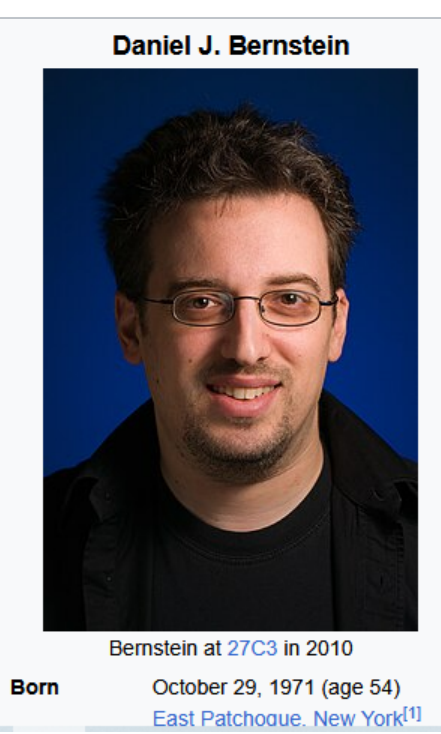
\includegraphics[width=48.30mm,height=201.96mm]{../../images/llm/page_079_img_01.png}%
\end{textblock*}

\end{document}
